% \documentclass[11pt,mathserif]{beamer}
\documentclass[11pt]{beamer}

\usepackage[english]{babel}
\usepackage{pgf}
\usepackage{amsmath,amssymb,wasysym}
\usepackage[latin1]{inputenc}
\usepackage{multirow}
\usepackage{graphicx}
\usepackage{ulem}
\usepackage{color}
\usepackage{comment}
\usepackage{hyperref}
\usepackage{listings}
\usepackage{tabularx}
\usepackage{verbatim}

%\lstnewenvironment{code}{\lstset{language=C,basicstyle=\scriptsize\ttfamily}}{}

\definecolor{dred}{RGB}{200,0,0}
\definecolor{dgreen}{RGB}{0,150,0}

\mode<presentation>
{
  \useinnertheme{rectangles}
  \useoutertheme{split}
  \setbeamerfont{block title}{size={}}
  \usefonttheme{structurebold}
  \usecolortheme{Intel}
  \setbeamercovered{transparent}
}

\pgfdeclareimage[width=3.0cm]{intel-logo}{intel2}
\titlegraphic{
  \pgfuseimage{intel-logo}
}

\title[MPI+MPI]{The MPI+MPI programming model and why we need shared-memory MPI libraries}
\author[Jeff Hammond]{Jeff Hammond}
\institute[Intel Labs]{Extreme Scalability Group \& Parallel Computing Lab\\ Intel Corporation (Portland, OR)}
\date[]{26 September 2014}

\begin{document}

\frame{\titlepage}

\begin{frame}{}
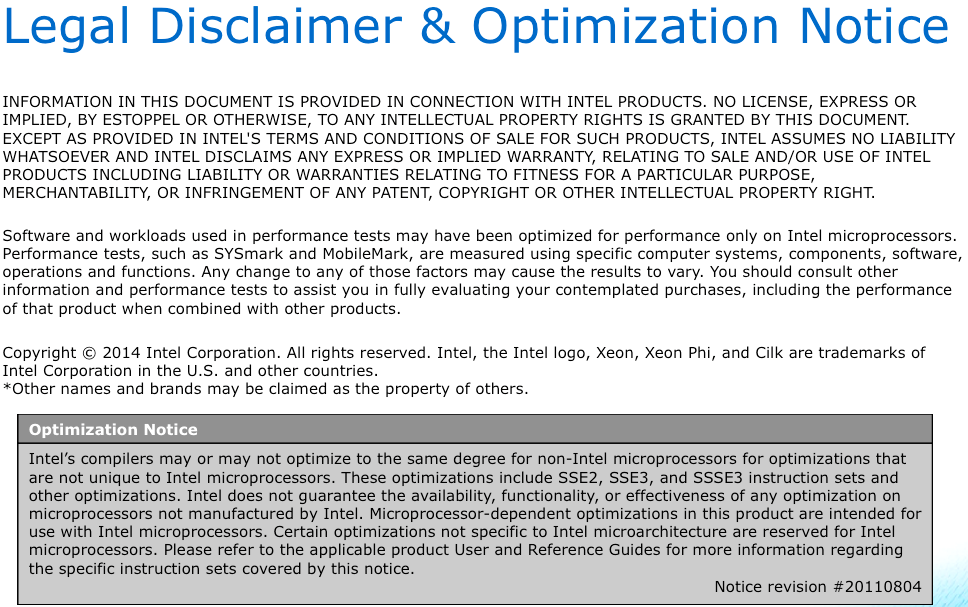
\includegraphics[scale=0.33,angle=0]{intel-legal} \
\end{frame}

\begin{frame}{Extreme Scalability Group Disclaimer}
    \begin{itemize}
        \item I work in Intel Labs and therefore don't know anything about Intel products.
        \item I work for Intel, but I am not an official spokesman for Intel.
              Hence anything I say are my words, not Intel's.
              Furthermore, I do not speak for my collaborators,
              whether they be inside or outside Intel.
        \item You may or may not be able to reproduce any performance numbers I report.
        \item Performance numbers for non-Intel platforms were obtained by non-Intel people.
        \item Hanlon's Razor.
    \end{itemize}
\end{frame}

\begin{frame}{Abstract (for posterity)} \Large
    The MPI-3 standard provides a portable interface to interprocess 
    shared-memory through the RMA functionality. This allow applications 
    to leverage shared-memory programming within a strictly MPI paradigm, 
    which mitigates some of the challenges of MPI+X programming using 
    threads associated with shared-by-default behavior and race conditions, 
    NUMA and Amdahl's law. I will describe the MPI shared-memory capability 
    and how it might be targeted by existing multithreaded libraries.
\end{frame}

\begin{frame}{} \LARGE
  \begin{center}
      \textbf{MPI-3}
  \end{center}
\end{frame}

\begin{frame}{Quiz} \Large
    What is \textbf{MPI}? \\
    (A) A bulky, bulk-synchronous model. \\
    (B) The programing model of Send-Recv. \\
    (C) An explicit, CSP-like, private-address-space programming model. \\
    (D) An industry-standard runtime API encapsulating
        1-, 2- and $N$-sided blocking and nonblocking communication
        and a whole bunch of utility functions for library development. \\
    (E) The assembling language of parallel computing!!
\end{frame}

\begin{frame}{The MPI You Know}
    \begin{tt}
        MPI\_Init(..); \\
        MPI\_Comm\_size(..); MPI\_Comm\_rank(..); \\
        MPI\_Barrier(..); MPI\_Bcast(..); \\
        MPI\_Reduce(..); MPI\_Allreduce(..); \\
        MPI\_Gather(..); MPI\_Allgather(..); \\
        MPI\_Scatter(..); MPI\_Alltoall(..); \\
        MPI\_Reduce\_scatter(..); MPI\_Reduce\_scatter\_block(..); \\
        MPI\_Send(..); MPI\_Recv(..); /* [b,nb] x [r,s,b] */ \\
        \ldots \\
        MPI\_Finalize();
    \end{tt}
\end{frame}

\begin{frame}{The MPI You Have Heard of But Don't Use}
    \begin{tt}
        MPI\_Ibarrier(..); MPI\_Ibcast(..); \\
        MPI\_Ireduce(..); MPI\_Iallreduce(..); \\
        MPI\_Igather(..); MPI\_Iallgather(..); \\
        MPI\_Iscatter(..); MPI\_Ialltoall(..); \\
        MPI\_Ireduce\_scatter(..); MPI\_Ireduce\_scatter\_block(..); \\
    \end{tt}
    \vskip5ex
    Go forth a write bulk-asynchronous code!
\end{frame}

\begin{frame}{The MPI You Don't Know But Should}
    \begin{tt}
        MPI\_Comm\_create\_group(..); \\
        MPI\_Icomm\_dup(..); \\
        \ldots \\
        MPI\_Dist\_graph\_create\_adjacent(..); \\
        MPI\_Neighborhood\_allgather(..); \\
        MPI\_Neighborhood\_allgatherv(..); \\
        MPI\_Neighborhood\_alltoall(..); \\
    \end{tt}
    \vskip2ex
    Virtual topologies corresponding to algorithmic topology;
    additional semantic information enables MPI to optimize.
\end{frame}

\begin{frame}{The MPI You Don't Know and Might Not Want To}
    \begin{tt}
        Win\_create(..); Win\_allocate(..); \\
        Win\_allocate\_shared(..); Win\_shared\_query(..); \\
        Win\_create\_dynamic(..); Win\_attach(..); Win\_detach(..); \\
        Put(..); Get(..); Accumulate(..); \\
        Fetch\_and\_op(..); Compare\_and\_swap(..); \\
        Win\_lock(..); Win\_lock\_all(..); \\
        Win\_flush(\_local)(\_all)(..); Win\_sync(..); \\
        \ldots
    \end{tt}
    \vskip2ex
    MPI-3 is a superset of ARMCI and OpenSHMEM\ldots
    \vskip2ex
    \href{http://wiki.mpich.org/armci-mpi/}{http://wiki.mpich.org/armci-mpi/} \\
    \href{https://github.com/jeffhammond/oshmpi/}{https://github.com/jeffhammond/oshmpi/}
\end{frame}

\begin{frame}{Shared Memory implementations} \large
    What is MPI\_Win\_allocate\_shared(..)?
    \vskip1ex
    Historically, SysV shared memory used, but painfully.
    \vskip1ex
    POSIX shared memory good, but Windows, BSD/Mach\ldots
    \vskip1ex
    In HPC, we have XPMEM (Cray and SGI).  And BGQ\ldots
    \vskip1ex
    MPI processes can be threads, in which case, all is shared.
    \vskip1ex
    The purpose of MPI is to standardize best practice!
    \vskip1ex
    Shared-memory is a ``best practice.''
\end{frame}

\begin{frame}{MPI-3 Shared Memory}\Large
    Limitations: \\
    \begin{itemize}
        \item Only defined for cache-coherent systems (WIN\_MODEL=UNIFIED).
        \item Allocated collectively.
        \item Memory allocated contiguously \textit{by default}.
    \end{itemize}
    Features: \\
    \begin{itemize}
        \item It's SHARED MEMORY: what don't you love?
        \item Works together with RMA ops (e.g. atomics).
        \item Noncontiguous allocation upon request (hint).
    \end{itemize}
\end{frame}

\begin{frame}{} \LARGE
  \begin{center}
      \textbf{MPI+X}
  \end{center}
\end{frame}

\begin{frame}[fragile]{The future is MPI+X (supposedly)} \large
\begin{itemize}
	\item MPI+OpenMP is too often fork-join.
	\item Pthreads scare people; can't be used from Fortran (easily).
	\item Intel$^\circledR$ has Cilk$^\circledR$ and TBB.
	\item OpenCL is not a good model for application programmers
          and has no magic for portable performance (since such magic does not exist).
	\item CUDA$^\circledR$ is an X for only one type of hardware (ignoring Ocelot).
\end{itemize}
Never confuse portability with portable performance!
\end{frame}

\begin{frame}{Using MPI+OpenMP effectively} \Large 
\begin{itemize}
	\item Private data should behave like MPI but with load-store for comm.
	\item Shared data leads to cache reuse but also false sharing.
	\item NUMA is going to eat you alive.  BG is a rare exception.
	\item OpenMP offers little to no solution for NUMA.
	\item If you do everything else right, Amdahl is going to get you.
\end{itemize}
Intranode Amdahl and NUMA are giving OpenMP a bad name;
fully rewritten hybrid codes that exploit affinity behave very different
from MPI codes evolved into MPI+OpenMP codes.
\end{frame}

\begin{frame}{Fork-Join vs. Parallel-Serialize}
  \begin{center}
    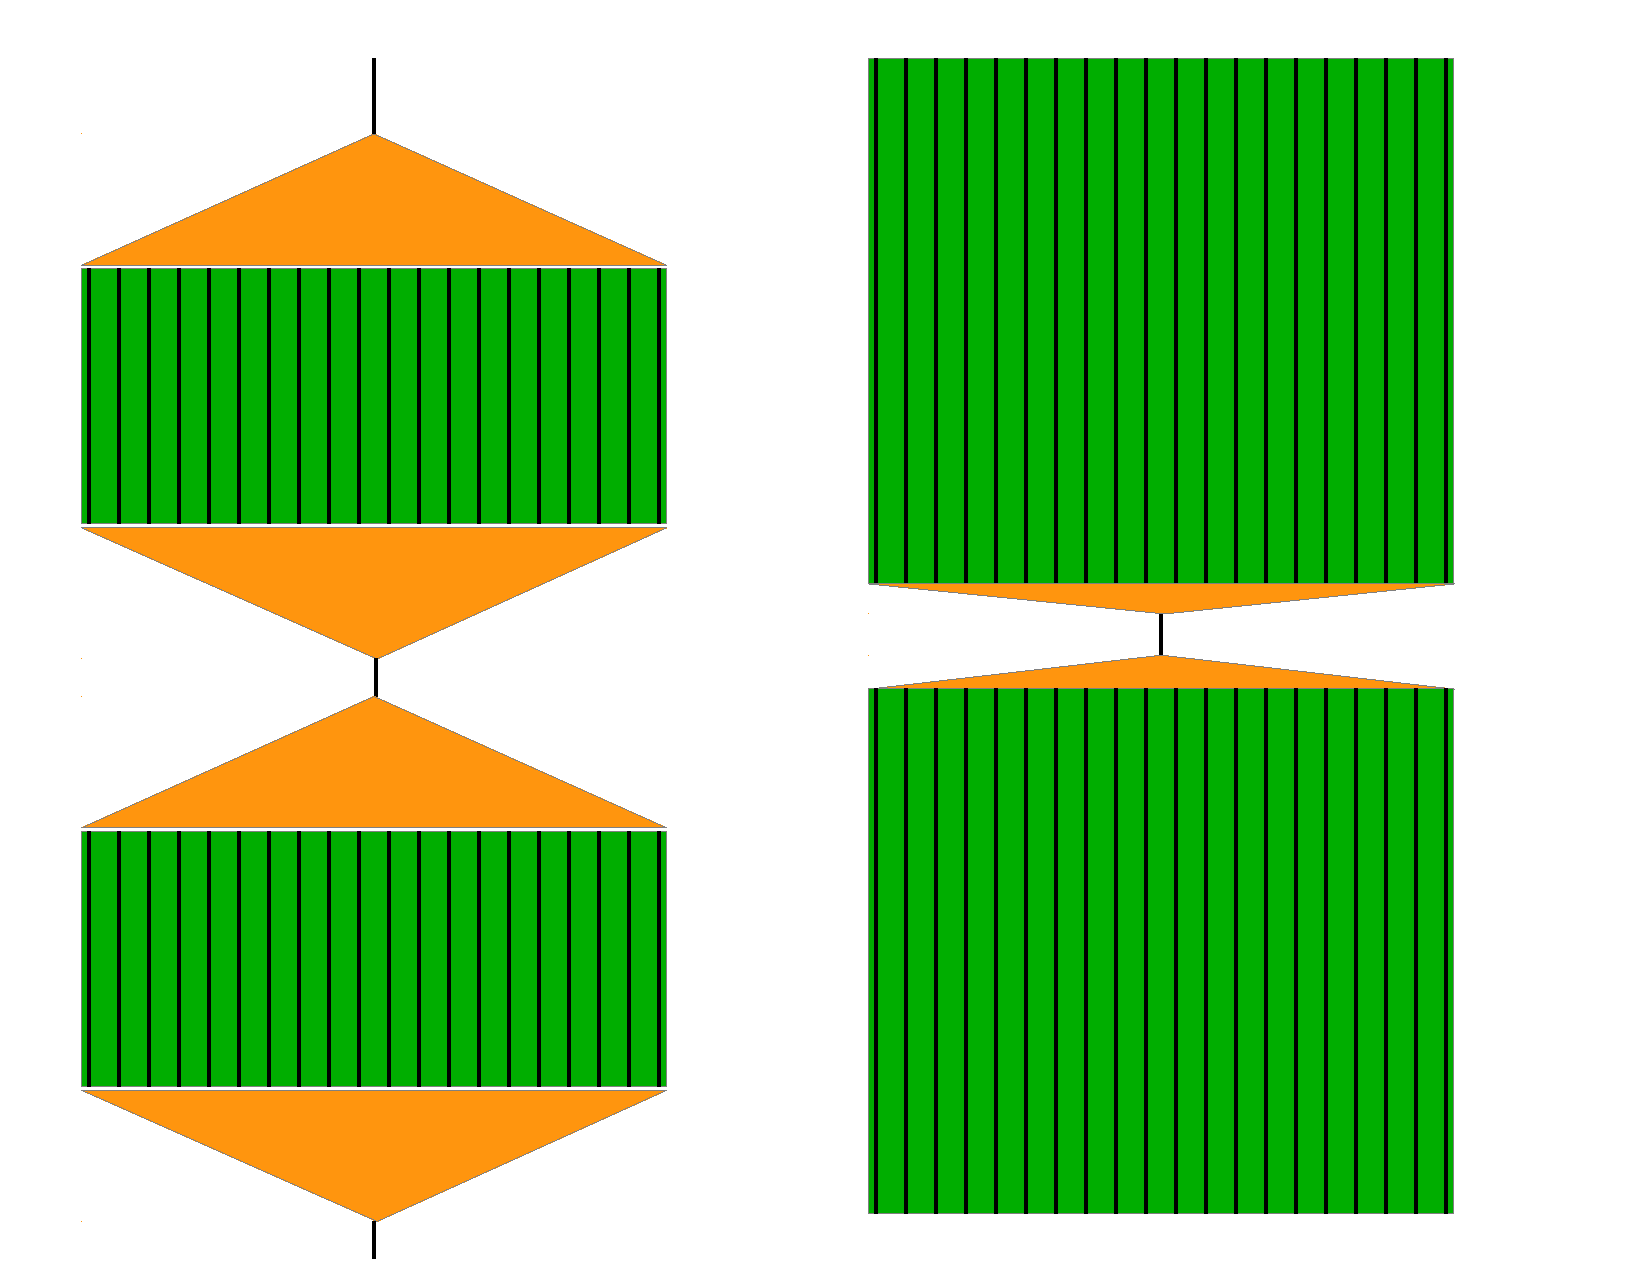
\includegraphics[scale=0.3,angle=0]{ForkJoin.pdf}
  \end{center}
\end{frame}

\begin{frame}{Fork-Join vs. Parallel-Serialize}
  \begin{columns}[T]
    \begin{column}{0.5 \linewidth}
      \begin{tt}
       \color{black}
       \#pragma omp parallel       \\
       \{ \\
       \color{green}
       /* thread-safe */      \\
       \vskip1ex
       \color{black}
       \#pragma omp single         \\
       \color{red}
       /* thread-unsafe */    \\
       \vskip1ex
       \color{black}
       \#pragma omp parallel for   \\
       \color{green}
       /* threaded loops */ \\
       \vskip1ex
       \color{black}
       \#pragma omp sections       \\
       {\color{green}
       /* threaded work */}  \\
       \}     \\
      \end{tt}
    \end{column}
    \begin{column}{0.5 \linewidth}
      \begin{tt}
       {\color{red} /* thread-unsafe */ }  \\
       \vskip1ex
       \color{black}
       \#pragma omp parallel for \\
       \{ \\
       {\color{green} /* threaded loops */} \\
       \} \\
       \vskip1ex
       {\color{red} /* thread-unsafe */ }  \\
       \vskip1ex
       \color{black}
       \#pragma omp parallel for \\
       \{ \\
       {\color{green} /* threaded loops */ } \\
       \} \\
       \vskip1ex
       \color{red}
       /* thread-unsafe work */  \\
      \end{tt}
    \end{column}
  \end{columns}
\end{frame}

\begin{frame}[fragile]{NUMA}
%See \texttt{./src/omp/numa.c} % where is this code?
\begin{verbatim}
> for n in 1e6 1e7 1e8 1e9 ; do ./numa.x $n ; done
n = 1000000    a: 0.009927 b: 0.009947 
n = 10000000   a: 0.018938 b: 0.011763 
n = 100000000  a: 0.123872 b: 0.072453 
n = 1000000000 a: 0.915020 b: 0.811122 
\end{verbatim}
The first-order effect requires a multi-socket system.
\vskip1ex
For more complicated data access patterns, you may see this even with parallel initialization.  
%In this case, consider (1) hiding latency, (2) not being bandwidth bound, and (3) task parallelism.
\end{frame}

\begin{frame}{} \LARGE
  \begin{center}
      \textbf{MPI$\otimes$X}
  \end{center}
\end{frame}

\begin{frame}{MPI$\otimes$X} \large 
\begin{itemize}
    \item Threads are independent, long-lived tasks in a shared address space.
    \item Threads all access MPI like they own it.
    \item \texttt{MPI\_THREAD\_MULTIPLE} is non-trivial overhead.
    \item Be sure you have a communicator per thread with collectives\ldots
    \item If your low-level network stack is not thread-safe\ldots
    \item God help you if you want to mix more than one threading model!$^{1}$
\end{itemize}
\vskip1ex
{\small $^{1}$ See \url{https://www.ieeetcsc.org/activities/blog/challenges_for_interoperability_of_runtime_systems_in_scientific_applications} }
\end{frame}

\begin{frame}{} \LARGE
  \begin{center}
      \textbf{MPI+MPI}
  \end{center}
\end{frame}

\begin{frame}{Best of all worlds?}
    MPI-1 between nodes; MPI-Shm within the node\ldots
    \begin{itemize}
        \item Private by default; shared by request.  Safe.
        \item Memory affinity to each core; NUMA issues should be rare.
        \item No fork-join - end-to-end parallel execution, 
              just a question of replicated or distributed (GA-like).
        \item No need to reimplement \textit{any} collectives.
        \item Easily supports both task- and data-parallelism.
        \item Hierarchy via MPI communicators.
        \item One runtime to rule them all.  No interop BS.
        \item \texttt{MPI\_THREAD\_SINGLE} sufficient.
    \end{itemize}
\end{frame}

\begin{frame}{Why not MPI+MPI?} \Large
    \begin{itemize}
        \item MPI shm allocation collective.
        \item MPI shm allocator not \texttt{malloc}.
        \item No cure for data races.
        \item Data races not cured.
        \item cured. races not Data
        \item All the intranode libraries use threads!!!
    \end{itemize}
\end{frame}

\begin{frame}{MPI-Shm libraries 1} \large
    \textbf{BLIS} should be the first MPI-Shm library:
    \begin{itemize}
        \item BLIS thread communicator maps perfectly to MPI communicator.
        \item Need to put BLIS communicator outside of API calls,
              but that's the only major change I can see.
        \item Tyler's implementation with OpenMP is trivially mapped
              to MPI calls.
        \item API refactoring for this is incredibly useful in threading
              models for task-parallelism and batching.
    \end{itemize}
\end{frame}

\begin{frame}{MPI-Shm libraries 2} \large
    \textbf{Elemental} should be the second MPI-Shm library:
    \begin{itemize}
        \item Does OpenMP really meet the needs of Elemental within a node?
        \item Lots of people don't want to think about hybrid, just MPI-only.
        \item Elemental with MPI-Shm within node could compete with threaded
              libraries and might beat them because of well-known fork-join
              issues in LAPACK.
        \item DistMatrix object hides all of the allocation issues internally,
              as it's already collective.
        \item We have an MPI-3 RMA AXPY implementation as a related proof-of-concept.
    \end{itemize}
\end{frame}

\begin{frame}{} \LARGE
  \begin{center}
      \textbf{MPI is dead.  Long live MPI!}
  \end{center}
\end{frame}

\begin{frame}{Acknowledgements} \Large
    Tyler Smith and Jed Brown, for explaining and discussing thread communicators at length.
    \vskip1ex
    Jack Poulson, for Elemental discussions over the years.
    \vskip1ex
    NUMA and Amdahl's Law, for holding OpenMP back and keeping MPI-only competitive in spite
    of the ridiculous cost of Send-Recv within a shared-memory domain.
\end{frame}

\end{document}
